% ============================================================
%  Příprava na maturitu – Elektrotechnika
%  Okruh 20: Užití elektrické energie a bezpečnost
% ============================================================

\documentclass[a4paper,10pt]{article}

\usepackage[T1]{fontenc}
\usepackage[utf8]{inputenc}
\usepackage[left=2.0cm, right=1.8cm, top=1.8cm, bottom=1.8cm]{geometry}
\usepackage{parskip}
\usepackage{xcolor}
\usepackage{tabularx}
\usepackage{booktabs}
\usepackage{tikz}
\usepackage{mdframed}
\usepackage{amsmath}
\usepackage{enumitem}
\usepackage{circuitikz}

\usetikzlibrary{arrows.meta, positioning, decorations.pathmorphing, shapes.geometric, calc}

% --- Barvy ---
\definecolor{accent}{HTML}{1A3A5C}
\definecolor{lightblue}{HTML}{EAF2F8}
\definecolor{lightyellow}{HTML}{FDFBE4}
\definecolor{lightgreen}{HTML}{EAF7EA}
\definecolor{lightred}{HTML}{FDE8E8}
\definecolor{lightgray}{HTML}{F4F4F4}

% --- Boxy ---
\newmdenv[backgroundcolor=lightblue,linecolor=accent!40,roundcorner=4pt,
  innertopmargin=6pt,innerbottommargin=6pt,innerleftmargin=8pt,innerrightmargin=8pt]{pojmybox}
\newmdenv[backgroundcolor=lightyellow,linecolor=accent!30,roundcorner=4pt,
  innertopmargin=6pt,innerbottommargin=6pt,innerleftmargin=8pt,innerrightmargin=8pt]{vysvetlenibox}
\newmdenv[backgroundcolor=lightgreen,linecolor=accent!40,roundcorner=4pt,
  innertopmargin=6pt,innerbottommargin=6pt,innerleftmargin=8pt,innerrightmargin=8pt]{vzorcebox}
\newmdenv[backgroundcolor=lightred,linecolor=accent!30,roundcorner=4pt,
  innertopmargin=6pt,innerbottommargin=6pt,innerleftmargin=8pt,innerrightmargin=8pt]{durazbox}

\setlist[itemize]{noitemsep, leftmargin=1.4em, topsep=2pt}
\setlist[enumerate]{noitemsep, leftmargin=1.4em, topsep=2pt}

% --- Zkratka pro jednotky ---
\newcommand{\jednotka}[1]{\,[\mathrm{#1}]}

\begin{document}

% ============================================================
\section*{\large Okruh 20 – Užití elektrické energie a bezpečnost}

\begin{pojmybox}
\textbf{Klíčové pojmy:}
bezpečné napětí a proud, účinky proudu na organismus, první pomoc, ochrana před úrazem (živé/neživé části), třídy ochrany spotřebičů, krytí IP, zóny v koupelnách, revize
\end{pojmybox}

\begin{vysvetlenibox}

% ================================================================
\subsection*{1. Účinky elektrického proudu na lidský organismus}

Lidské tělo je vodič (díky obsahu vody a solí). Průchod proudu tělem může mít tepelné, chemické nebo fyziologické účinky.

\textbf{Mezní hodnoty (AC 50 Hz):}
\begin{itemize}
    \item \textbf{0,5 mA:} Práh vnímání (mírné brnění).
    \item \textbf{10 mA:} Práh uvolnění (křeče, člověk se již nedokáže sám pustit vodiče).
    \item \textbf{30 mA:} Práh nebezpečí (křeče dýchacích svalů, při delším působení smrt).
    \item \textbf{100 mA a více:} Fibrilace srdečních komor, smrtelný úraz.
\end{itemize}

\begin{vzorcebox}
Odpor lidského těla se pro účely bezpečnosti uvažuje cca \textbf{1000 $\Omega$} (mezi rukou a nohou). Proud protékající tělem určíme z Ohmova zákona $I = U / R_{t\check{e}lo}$.
\end{vzorcebox}

% ================================================================
\subsection*{2. Dovolená bezpečná napětí}

Bezpečné napětí závisí na prostředí (suché, vlhké, mokré) a na tom, zda jde o dotyk živých nebo neživých částí.

\begin{center}
\begin{tabularx}{0.85\linewidth}{@{} l X X @{}}
\toprule
\textbf{Prostředí} & \textbf{Střídavé (AC)} & \textbf{Stejnosměrné (DC)} \\
\midrule
Normální a suché & 50 V & 120 V \\
Vlhké & 25 V & 60 V \\
Mokré (bazény, vany) & 12 V & 25 V \\
\bottomrule
\end{tabularx}
\end{center}

% ================================================================
\subsection*{3. Ochrana před úrazem elektrickým proudem}

\begin{itemize}
    \item \textbf{Ochrana před dotykem ŽIVÝCH částí (základní):} Izolace, kryty, zábrany, poloha (mimo dosah).
    \item \textbf{Ochrana při PORUŠE (dotyk neživých částí):} Automatické odpojení od zdroje (jistič, chránič + uzemnění), dvojitá izolace, elektrické oddělení (trafo), malé napětí (SELV/PELV).
\end{itemize}

% ================================================================
\subsection*{4. Třídy ochrany elektrických spotřebičů}

Každý spotřebič musí mít označení, do které třídy ochrany spadá:

\begin{itemize}
    \item \textbf{Třída 0:} Pouze základní izolace. \textbf{V ČR zakázáno!}
    \item \textbf{Třída I:} Má základní izolaci a neživé části (kovový kryt) jsou připojeny k \textbf{ochrannému vodiči PE} (zeleno-žlutý). Přívodní šňůra má 3 dráty. \textit{Symbol: značka uzemnění.}
    \item \textbf{Třída II:} Má \textbf{dvojitou nebo zesílenou izolaci}. Nepotřebuje a nesmí být připojen k vodiči PE. Přívodní šňůra má 2 dráty. \textit{Symbol: dva čtverce v sobě.}
    \item \textbf{Třída III:} Spotřebič pracuje s \textbf{bezpečným malým napětím} (SELV/PELV), které nemůže způsobit úraz. \textit{Symbol: kosočtverec s římskou III.}
\end{itemize}

\begin{center}

\begin{tikzpicture}[thick, scale=0.8]
  % Symbol Třída II
  \draw (0,0) rectangle (1.2,1.2);
  \draw (0.2,0.2) rectangle (1,1);
  \node[below] at (0.6, -0.2) {Třída II};

  % Symbol Třída III
  \begin{scope}[xshift=4cm, yshift=0.6cm]
    \draw (0,0) -- (0.8,0.8) -- (1.6,0) -- (0.8,-0.8) -- cycle;
    \node at (0.8,0) {III};
    \node[below] at (0.8, -1) {Třída III};
  \end{scope}
\end{tikzpicture}
\end{center}

% ================================================================
\subsection*{5. Stupně krytí IP (Ingress Protection)}

Udává odolnost zařízení proti vniknutí cizích těles (prachu) a vody. Značí se \textbf{IPxx}.
\begin{enumerate}
    \item \textbf{První číslice (0–6):} Ochrana před dotykem a vniknutím prachu (6 = prachotěsné).
    \item \textbf{Druhá číslice (0–9):} Ochrana před vodou (4 = stříkající voda, 7 = dočasné ponoření, 8 = trvalé ponoření).
\end{enumerate}
\textit{Příklad: Zásuvka v koupelně musí mít aspoň IP44.}

% ================================================================
\subsection*{6. Bezpečnost v koupelnách (Zóny)}

V prostorách s vanou nebo sprchou je zvýšené riziko úrazu (voda snižuje odpor těla).

\begin{center}
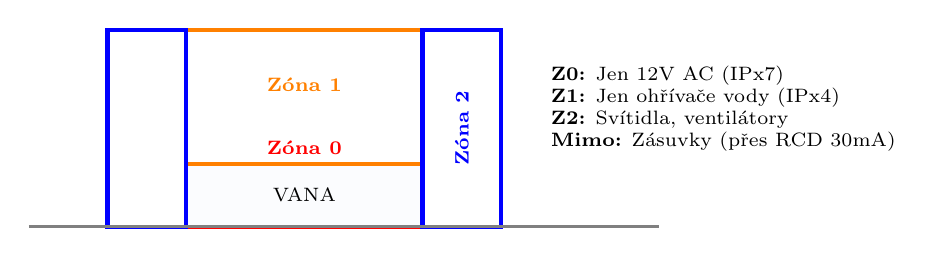
\begin{tikzpicture}[font=\scriptsize, thick]
  % Vana
  \draw[fill=lightblue!20] (0,0) rectangle (3,0.8);
  \node at (1.5,0.4) {VANA};

  % Zóna 0 (vnitřek vany)
  \draw[red, line width=1.5pt] (0,0) rectangle (3,0.8);
  \node[red] at (1.5, 1) {\textbf{Zóna 0}};

  % Zóna 1 (nad vanou do 225cm)
  \draw[orange, line width=1.5pt] (0,0.8) rectangle (3,2.5);
  \node[orange] at (1.5, 1.8) {\textbf{Zóna 1}};

  % Zóna 2 (60cm od vany)
  \draw[blue, line width=1.5pt] (3,0) rectangle (4,2.5);
  \draw[blue, line width=1.5pt] (0,0) rectangle (-1,2.5);
  \node[blue, rotate=90] at (3.5, 1.25) {\textbf{Zóna 2}};

  % Podlaha
  \draw[gray] (-2,0) -- (6,0);
  
  \node[align=left, anchor=west] at (4.5, 1.5) {
    \textbf{Z0:} Jen 12V AC (IPx7)\\
    \textbf{Z1:} Jen ohřívače vody (IPx4)\\
    \textbf{Z2:} Svítidla, ventilátory\\
    \textbf{Mimo:} Zásuvky (přes RCD 30mA)
  };
\end{tikzpicture}
\end{center}

% ================================================================
\subsection*{7. První pomoc při úrazu elektrickým proudem}

\begin{enumerate}
    \item \textbf{Vlastní bezpečnost:} Nedotýkat se postiženého, dokud je pod proudem!
    \item \textbf{Přerušení proudu:} Vypnout vypínač, jistič, nebo odsunout vodič nevodivým předmětem (dřevo).
    \item \textbf{Kontrola stavu:} Pokud postižený nedýchá $\implies$ \textbf{resuscitace} (30 stlačení hrudníku, 2 vdechy).
    \node[right] at (0,-1) {\textbf{Vždy volat 155!}};
\end{enumerate}

\begin{durazbox}
\textbf{Revize:} Každé elektrické zařízení (instalace v budovách i spotřebiče v práci) musí procházet pravidelnými revizemi prováděnými revizním technikem. Cílem je ověřit stav izolace a funkčnost ochran (zejména odpor ochranného vodiče a vybavovací proud chrániče).
\end{durazbox}

\end{vysvetlenibox}

\end{document}